\documentclass[11pt]{article}

\usepackage{fullpage}
\usepackage{graphicx}
\usepackage{amsmath}
\usepackage{amssymb}
\usepackage{amsthm}
\usepackage{fancyvrb}

\parindent0in
\pagestyle{plain}
\thispagestyle{plain}

\newcommand{\myname}{Mehshan Mustafa}
\newcommand{\dated}{\today}

\newenvironment{theorem}[2][Theorem]{\begin{trivlist}
\item[\hskip \labelsep {\bfseries #1}\hskip \labelsep {\bfseries #2.}]}{\end{trivlist}}
\newenvironment{lemma}[2][Lemma]{\begin{trivlist}
\item[\hskip \labelsep {\bfseries #1}\hskip \labelsep {\bfseries #2.}]}{\end{trivlist}}
\newenvironment{exercise}[2][Exercise]{\begin{trivlist}
\item[\hskip \labelsep {\bfseries #1}\hskip \labelsep {\bfseries #2.}]}{\end{trivlist}}
\newenvironment{problem}[2][Problem]{\begin{trivlist}
\item[\hskip \labelsep {\bfseries #1}\hskip \labelsep {\bfseries #2.}]}{\end{trivlist}}
\newenvironment{question}[2][Question]{\begin{trivlist}
\item[\hskip \labelsep {\bfseries #1}\hskip \labelsep {\bfseries #2.}]}{\end{trivlist}}
\newenvironment{corollary}[2][Corollary]{\begin{trivlist}
\item[\hskip \labelsep {\bfseries #1}\hskip \labelsep {\bfseries #2.}]}{\end{trivlist}}
\newenvironment{solution}{\begin{proof}[Solution]}{\end{proof}}
\newenvironment{idea}[2][Proof Idea.]{\textit{#1} #2}

\begin{document}
\textbf{Introduction to the Theory of
Computation}\hfill\textbf{\myname}\\[0.01in]
\textbf{Chapter 1: Reqular Languages}\hfill\textbf{\dated}\\
\smallskip\hrule\bigskip

\begin{problem}{1.39}
The construction in Theorem 1.54 shows that every GNFA is equivalent to a GNFA with only two states. We can show that an opposite phenomenon occurs for DFAs. Prove that for every $k > 1$, a language $A_{k} \subseteq \{0,1\}^{*}$ exists that is recognized by a DFA with k states but not by one with only $k-1$ states.
\end{problem}

\begin{proof}
Let $A_{k}$ be the language of all strings of length at least $k-1$.
\[ A_{k} = \{ w \ | \ w \in \{0, 1\}^{*} \ and \ |w| \geq k-1 \} \]
\[ w = w_{1}w_{2}w_{3} \cdots w_{k-1} \cdots w_{n}, \ where \ n \geq k-1 \]
The state diagram of a DFA $D_{k}$ that recognizes $A_{k}$ with $k$ states is given below. Each symbol $w_{i}$, where $1 \leq i \leq k-1$, requires a transition between two states $q_{i}$ and $q_{i+1}$. To construct a new DFA $D_{k-1}$ that recognizes $A_{k}$ with $k-1$ states by using $D_{k}$, there are three options:
\begin{enumerate}
\item Remove state $q_{1}$ and make $q_{2}$ the start state. First symbol $w_{1}$ is skipped. 
\item Remove state $q_{k}$, make $q_{k-1}$ the accept state and add a new transition from $q_{k-1}$ to $q_{k-1}$ for symbols 0 and 1. Symbol $w_{k-1}$ is skipped. 
\item Remove any intermediate state $q_{i}$, where $1 < i < k$, and add a new tranisition for symbols 0 and 1 from state $q_{i-1}$ to $q_{i+1}$. Symbol $w_{i}$ is skipped. 
\end{enumerate}
In all three cases the minimum length of strings, which are recognized by the DFA $D_{k-1}$ is reduced by one. Therefore, there does not exist a DFA that recognizes $A_{k}$ with $k-1$ states.
\begin{center}
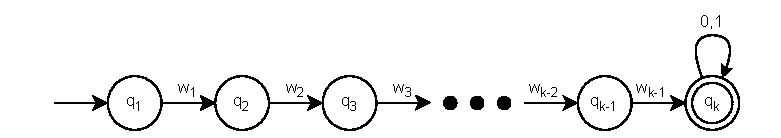
\includegraphics[scale=1.0]{Figures/Problem1.39.pdf} \\
State diagrams of DFA $D_{k}$ that recognizes $A_{k}$. Each $w_{i} \in \{0,1\}$.
\end{center}
\end{proof}
\end{document}